\documentclass{beamer}
\usepackage[utf8x]{inputenc}
\usepackage{amsmath, amsfonts, epsfig, xspace}
\usepackage{algorithm,algorithmic}
\usepackage{pstricks,pst-node}
\usepackage{multimedia}
\usepackage[normal,tight,center]{subfigure}
\setlength{\subfigcapskip}{-.5em}
\usepackage{beamerthemewarsaw}

\PrerenderUnicode{ö}
\PrerenderUnicode{ó}
\author[Jordi Böhme López, Manuel Woelker]{Jordi Böhme López, Manuel Woelker}

\title[Down with war!\hspace{2em}\insertframenumber/\inserttotalframenumber]{Down with war!}
\subtitle{Server-side deployment with p2}

\date{March 25, 2009} %leave out for today's date to be insterted

%\institute{EclipseSource}

\begin{document}

\maketitle

% \section{Introduction}  % add these to see outline in slides

\begin{frame}
  \frametitle{Status quo: Classic web application}
\begin{figure}
   \includegraphics[width=0.9\textwidth]{diagrams/stack_svg_p0.pdf}
\end{figure}
\end{frame}

\begin{frame}
  \frametitle{Status quo: Classic OSGi web application}
\begin{figure}
   \includegraphics[width=0.9\textwidth]{diagrams/stack_svg_p1.pdf}
\end{figure}
\end{frame}

\begin{frame}
  \frametitle{Status quo: Problems}
  \begin{itemize}
  \item Monolithic blobs\pause
  \item hard to reconfigure or update parts\pause
  \item hard to replace parts\pause
  \item orthogonal options lead to exponential growth\pause
  \item no included distribution mechanism
  \end{itemize}   
\end{frame}

\begin{frame}
  \frametitle{Deployment Wishlist}
  \begin{itemize}
  \item modular system\pause
  \item flexible\pause
  \item automatic dependency management\pause
  \item proven mechanisms\pause
  \item using existing technology
  \end{itemize}   
\end{frame}

\begin{frame}
  \frametitle{Example: Hudson Plugins}
\begin{columns}
\column{2in}
  \begin{itemize}
  \item more than 100 plugins\pause
  \item "proprietary" plugin system\pause
  \item hand-crafted\pause
  \end{itemize}   
\column{2.5in}
\onslide<1->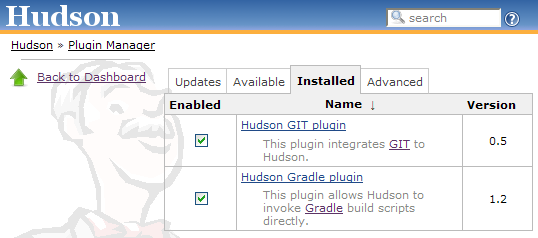
\includegraphics[width=1.0\textwidth]{hudson.png}
\end{columns}
\end{frame}


\begin{frame}
  \frametitle{Easier solution: p2}
  \begin{itemize}
  \item works well on the desktop\pause
  \item pulls in dependencies\pause
  \item prevents conflicts\pause
  \item much more general than one might think\pause
  \item powerful: mirroring, different protocols, proxy configuration, reusing locally cached bundles
  \end{itemize}   
\end{frame}

\begin{frame}
  \frametitle{P2 "Cold-deploy"}
\begin{figure}
   \includegraphics[width=0.9\textwidth]{diagrams/stack_svg_p2.pdf}
\end{figure}
\end{frame}

\begin{frame}
  \frametitle{P2 "Cold-deploy"}
\begin{columns}
\column{2in}
  \begin{itemize}
  \item p2 not inside framework\pause
  \item but maybe in another webapp\pause
  \item server restart after deployment\pause
  \item very robust
  \end{itemize}      
\column{2.5in}
\onslide<1->\includegraphics[width=1.0\textwidth]{diagrams/stack_svg_p2.pdf}
\end{columns}
\end{frame}

\begin{frame}
  \frametitle{P2 "Hot-deploy"}
\begin{figure}
   \includegraphics[width=0.9\textwidth]{diagrams/stack_svg_p3.pdf}
\end{figure}
\end{frame}

\begin{frame}
  \frametitle{P2 "Hot-deploy"}
\begin{columns}
\column{2in}
  \begin{itemize}
  \item p2 inside framework\pause
  \item better control of bundle life cycle\pause
  \item good for high-availability systems\pause
  \item not as resilient (Permgen, thread problems)
  \end{itemize}      
\column{2.5in}
\onslide<1->\includegraphics[width=1.0\textwidth]{diagrams/stack_svg_p3.pdf}
\end{columns}
\end{frame}


\begin{frame}
  \frametitle{Caveats}
  \begin{itemize}
  \item long running webapp process still problematic (permgen, threads again)\pause
  \item tooling \pause
  \item bootstrapping\pause
  \item appserver upgrades
  \end{itemize}   
\end{frame}

\begin{frame}
  \frametitle{Benefits}
  \begin{itemize}
  \item leveraging powerful dependency manager\pause
  \item dependencies are resolved and added automatically\pause
  \item incremental updates possible\pause
  \item good for modular or flexible deployments\pause
  \item no need for $2^n$ war versions\pause
  \item sophisticated distribution mechanisms
  \end{itemize}   
\end{frame}


 
\begin{frame}
  \frametitle{Outlook}
  \begin{itemize}
  \item works well with RAP \& Single Source applications\pause
  \item OSGi-based appservers (e.g. Glassfish)\pause
  \item "Rich server platform"
  \end{itemize}   
\end{frame}

\end{document}